\documentclass[
aps,prl,twocolumn,amsmath,amssymb,superscriptaddress,
longbibliography,floatfix
]{revtex4-2}

\usepackage{bm}
\usepackage{graphicx}
\usepackage{xcolor}
\usepackage[colorlinks=true,citecolor=blue!55!black,
urlcolor=blue!55!black,linkcolor=blue!55!black]{hyperref}

\graphicspath{{figs/}}
\setlength{\emergencystretch}{3em}

\newcommand{\bq}{\bm q}
\newcommand{\Szz}{S^{zz}}

\begin{document}

\title{Roton-like Reconstruction of the Emergent Photon in Quantum Spin Ice}

\author{Zhengbang Zhou}
\email{zhengbang.zhou@mail.utoronto.ca}
\affiliation{Department of Physics, University of Toronto,
Toronto, Ontario M5S 1A7, Canada}

\author{Yong Baek Kim}
\email{ybkim@physics.utoronto.ca}
\affiliation{Department of Physics, University of Toronto,
Toronto, Ontario M5S 1A7, Canada}

\date{\today}

\begin{abstract}
The emergent photon of quantum spin ice is well understood at long
wavelength, but its fate at lattice momenta---where the compact
spin-$\frac12$ gauge theory has no small parameter---has never been
resolved eigenstate by eigenstate. We compute the operator-resolved
$\Szz(\bq,\omega)$ of the pure pyrochlore ring-exchange model on 48-,
64-, 72-, and 96-site clusters, the largest a constrained sector of
dimension $1.47\times10^{8}$, and find five things. First, near the
zone-boundary $L$ point the spectrum reconstructs at order one: a
dominant level at $0.90$--$1.07K$ takes $50$--$54\%$ of the
longitudinal weight at roughly half the Gaussian-photon energy, while
a second level remains photon-like at $1.65$--$1.81K$. Second, the low
mode is microscopically distinct, gaining ring flippability where
nonreconstructing momentum classes at identical $|\bq|$ lose it.
Third, the effect is stable across four clusters, three cluster
shapes, and a factor $1.6\times10^{4}$ in Hilbert-space dimension,
with a scale-free branch ratio $\omega_{\rm low}/\omega_{\rm high}
=0.55$--$0.59$. Fourth, where it occurs is predicted before any
excited state is computed by the Feynman ratio $f_1(\bq)/S(\bq)$ of
oscillator strength to static structure factor, which discriminates
correctly between inequivalent $L$ classes on two clusters and locates
a second soft momentum away from $L$; sign-free Green's-function Monte
Carlo carries this ground-state diagnostic to complete momentum grids
of $2048$ spins, where the $L$-centered minimum persists with under
two percent drift. Fifth, the phenomenology is that of a lattice
roton and predicts a two-feature zone-boundary response---split by
nearly a factor of two, weighted two-to-one, both ratios independent
of the overall energy scale---that no single renormalized photon pole
can produce.
\end{abstract}

\maketitle

\emph{Introduction.}---Quantum spin ice realizes a compact $U(1)$
lattice gauge theory in a magnetic insulator. In the two-in--two-out
manifold of the pyrochlore lattice, virtual exchange resonates the six
spins around an elementary hexagon, and the resulting deconfined phase
supports a gapless emergent photon together with gapped electric and
magnetic charges~\cite{Hermele2004,Castelnovo2008,Gingras2014,
SavaryBalents2017,RauGingras2019,Broholm2020}. That long-wavelength
description is quantitatively established and motivates the search for
candidate materials~\cite{Benton2012,Shannon2012,KatoOnoda2015,
Ross2011,Sibille2018,Gaudet2019,Gao2019,Smith2022,Poree2025,Gao2025}.

At lattice momenta the same theory is a different problem. The
electric field is microscopically saturated, $E_\ell=S^z_\ell=\pm\frac12$,
so the usual electric term $\sum_\ell E_\ell^2$ is a constant inside
the constrained manifold and the ring dynamics constitute the entire
nonconstant Hamiltonian. The photon stiffness is generated, not bare,
and the emergent fine-structure constant is large~\cite{Pace2021}.
Nothing in this construction restricts the theory to small $\bq$: the
ring model is a lattice Hamiltonian with excitations throughout its
Brillouin zone, and the short-wavelength regime is precisely where the
interactions are strongest and least explored.

Existing numerics stop short of that regime in a specific sense.
Gaussian and semiclassical treatments expand about small flux and are
controlled in the infrared, though they already predict substantial
anharmonic renormalization and an interaction-induced splitting of the
transverse polarizations~\cite{Benton2012,Kwasigroch2017,Kwasigroch2020,
Szabo2019}. Quantum Monte Carlo with analytic continuation resolves
broadened lineshapes and finds zone-boundary weight beyond Gaussian
electrodynamics, but not individual eigenstates or their matrix
elements~\cite{Huang2018}. Constrained-space exact diagonalization has
reached 96 spins, organized around ground-state and low-energy
electrodynamic parameters rather than the full
response~\cite{Pace2021}. What has not been done is the direct
question: at large $|\bq|$, \emph{which} eigenstates of the compact
theory carry the spin response, and how much.

We answer it, and the answer is not a renormalized photon. Our
punchlines are: (i) near the zone-boundary $L$ point one collective
level takes over half of the longitudinal spectral weight at roughly
half the Gaussian-photon energy, while a second level remains
photon-like nearly a factor of two above it; (ii) the low mode is
microscopically distinct, gaining ring flippability where
nonreconstructing momentum classes at identical $|\bq|$ lose it;
(iii) the effect is stable across four clusters, three shapes, and
four orders of magnitude in Hilbert-space dimension, with a
scale-free branch ratio $0.55$--$0.59$; (iv) its location is
predicted from ground-state data alone through the Feynman ratio
$f_1/S$, which we verify as a forward diagnostic three times and
carry to $2048$ spins by sign-free Monte Carlo; and (v) the resulting
two-feature zone-boundary response is an experimentally
distinguishable alternative to a single renormalized photon pole.

\emph{Model, observable, and method.}---We study the standard ring
Hamiltonian in the spin-ice manifold~\cite{Hermele2004,Shannon2012},
$H=-K\sum_p(W_p+W_p^\dagger)$ with
$W_p=S_1^+S_2^-S_3^+S_4^-S_5^+S_6^-$ summed over contractible
elementary hexagons; in gauge language $W_p=e^{iB_p}$ and $H$ is the
compact magnetic energy $-2K\sum_p\cos B_p$. Because $S^z$ is the
emergent electric field, the natural probe is the sublattice-summed
longitudinal response
\begin{equation}
\Szz(\bq,\omega)=\frac1N\sum_{\mu,n}
\bigl|\langle n|S^z_\mu(\bq)|0\rangle\bigr|^2\,
\delta(\omega-\omega_n),
\label{eq:szz}
\end{equation}
with $S^z_\mu(\bq)=\sum_{i\in\mu}e^{-i\bq\cdot\bm r_i}S^z_i$. All
spectral fractions below are normalized within Eq.~(\ref{eq:szz}) at
fixed $\bq$. This is the theoretical pseudospin response, not a
material-specific neutron cross section, which additionally involves
coherent sublattice interference, the local easy axes, the $g$ tensor,
form factors, and the polarization projector; we return to this point
and treat it fully in the Supplemental Material.

We evaluate Eq.~(\ref{eq:szz}) by complete diagonalization at 48 sites
and by Lanczos continued fractions at 64, 72, and 96, the last in a
winding sector of dimension $146\,758\,352$. Winding sectors are
certified exhaustively at 48 and 72 sites---every one of the $155$ and
$310$ sectors diagonalized, with margins of $0.99K$---and by the
twelve largest of $519$ candidates at 96. Recomputing the 96-site
spectra at Krylov dimension $200$ rather than $120$ leaves the
dominant pole energies and residues unchanged to machine precision.
Cluster construction, momentum certification, gates, and convergence
are detailed in the Supplemental Material.

\emph{An unexpected low-energy mode.}---Figure~\ref{fig:dispersion}
shows the operator-resolved spectrum along
$\Gamma\!\to\!L\!\to\!(0,\frac12,\frac12)\!\to\!X\!\to\!\Gamma$. Near
$\Gamma$ the dominant response tracks the expected long-wavelength
photon. Near $L$ it does not. The spectrum reorganizes into two
dominant levels, and the lower one takes most of the weight
(Table~\ref{tab:ladder}). Fixing the single Gaussian energy scale from
the long-wavelength spectrum places the Gaussian photon at $L$ near
$2.03K$; the low mode sits at roughly half of that, while its partner
sits at $81$--$89\%$, the magnitude of renormalization an ordinarily
interacting photon exhibits.

Throughout we call these two levels simply the \emph{lower} and
\emph{upper branch}. The terminology is operational: at each momentum
the $S^z$ probe lives in a two-dimensional transverse subspace of the
gauge field, and the two dominant levels couple through nearly
orthogonal directions of that subspace, so they are the two
independent collective features the probe can create there. No
adiabatic connection to a free photon is implied by either name; with
$E^2$ a c-number there is no coupling constant to turn off, and hence
no such connection to construct.

\begin{figure*}[t]
\centering
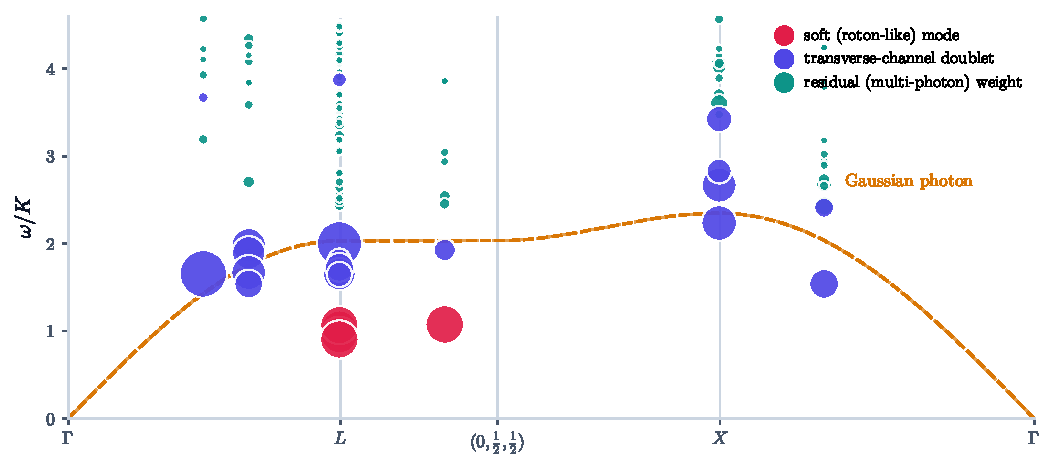
\includegraphics[width=0.98\textwidth]{fig_dispersion.pdf}
\caption{\textbf{Order-one reconstruction at lattice momentum.}
Operator-resolved $S^z$ spectrum along
$\Gamma\!\to\!L\!\to\!(0,\frac12,\frac12)\!\to\!X\!\to\!\Gamma$,
combining all four diagonalized clusters; marker area is the fraction
of the sublattice-summed weight carried by each level at its momentum.
Red marks the lower branch where it reconstructs, indigo the dominant
branches elsewhere, teal the residual weight. The dashed curve is the
Gaussian photon with a single fitted energy scale. The
long-wavelength response is photon-like; near $L$, and again at
$(\frac16,\frac12,\frac12)$ on the 72-site cluster, the lower branch
collapses to roughly half the Gaussian energy and absorbs half of the
response.}
\label{fig:dispersion}
\end{figure*}

\begin{table}[b]
\caption{The reconstruction across all four clusters. Weights are
fractions of $\Szz$ at the same momentum; $d\omega/dV$ is the
flippability census of Eq.~(\ref{eq:census}).}
\label{tab:ladder}
\begin{ruledtabular}
\begin{tabular}{lcccc}
sites & 48 & 64 & 72 & 96\\
\hline
sector dimension & $9104$ & $2.5{\times}10^5$ & $9.7{\times}10^5$
 & $1.5{\times}10^8$\\
$\omega_{\rm low}/K$ & $1.024$ & $0.954$ & $1.068$ & $0.904$\\
weight & $50.8\%$ & $50.0\%$ & $54.0\%$ & $54.4\%$\\
$\omega_{\rm high}/K$ & $1.730$ & $1.652$ & $1.814$ & $1.647$\\
weight & $32.3\%$ & $31.3\%$ & $17.8\%$ & $22.5\%$\\
$\omega_{\rm low}/\omega_{\rm high}$ & $0.592$ & $0.578$ & $0.589$
 & $0.549$\\
$d\omega_{\rm low}/dV$ & $+0.339$ & $+0.338$ & $+0.134$ & $+0.259$\\
\end{tabular}
\end{ruledtabular}
\end{table}

\emph{What the mode does that a photon does not.}---Two of its
properties are already in Table~\ref{tab:ladder}: it is
weight-dominant, carrying two to three times the response of its
partner, and it is anomalously soft while that partner is not. A
third is microscopic and uses no fitted energy scale. Adding the
standard Rokhsar--Kivelson term, $H(V)=H+V\sum_p n_p^{\rm flip}$ with
$n_p^{\rm flip}$ the projector onto a flippable alternating hexagon,
and applying Hellmann--Feynman at the physical point $V=0$ gives
\begin{equation}
\frac{d\omega_n}{dV}\Big|_{V=0}=
\Bigl\langle n\Bigl|\sum_p n_p^{\rm flip}\Bigr|n\Bigr\rangle-
\Bigl\langle 0\Bigl|\sum_p n_p^{\rm flip}\Bigr|0\Bigr\rangle,
\label{eq:census}
\end{equation}
an exact state-resolved census of the flippable hexagons the
excitation adds or removes. The ground state maximizes ring
resonance, so a typical excitation reduces flippability; averaged over
a sector the census is exactly $\mathrm{nnz}(H)/D-\langle
n^{\rm flip}\rangle_0<0$, and at 48 sites only $58$ of $9104$
eigenstates are positive.

The lower branch is positive at every size (Table~\ref{tab:ladder}):
it rearranges spins so that \emph{more} hexagons could flip while the
phases of those ring processes are less coherent, paying its energy in
resonance rather than in the ice rule. The sharpest form of the
statement is a comparison made within a single cluster. The
anisotropic 64- and 96-site boxes split the $L$ star into two
inequivalent classes at identical $|\bq|$ and identical Gaussian
energy; the class that reconstructs has census $+0.338$ and $+0.259$,
while the class that does not has $-0.166$ and $-0.015$, $-0.088$
(Fig.~\ref{fig:rk}). We claim no general sign rule: the upper
branch's census is negative at 48 and 64 but positive at 72 and 96,
and the census magnitudes are the least size-stable of our
diagnostics. It is the same-momentum class contrast, which requires
neither a fitted scale nor a comparison across sizes, that identifies
the reconstruction microscopically.

\begin{figure}[t]
\centering
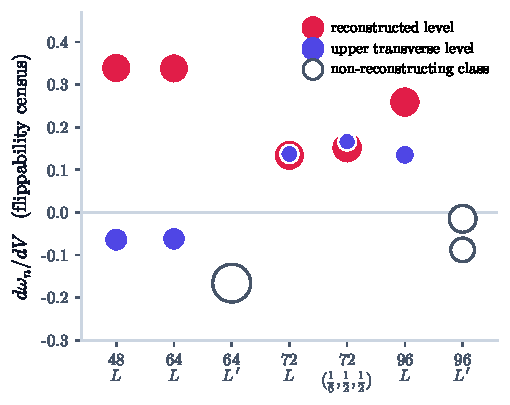
\includegraphics[width=\columnwidth]{fig_mechanism.pdf}
\caption{\textbf{Microscopic fingerprint.} Flippability census
[Eq.~(\ref{eq:census})] of the dominant levels. The robust statement
is the within-cluster contrast: on the anisotropic 64- and 96-site
clusters the lower branch of the reconstructing $L$ class is positive
while the dominant levels of the nonreconstructing class (open
symbols) at the same $|\bq|$ are negative. The upper branch's sign is
not itself a diagnostic; it is negative at 48 and 64 and positive at
72 and 96.}
\label{fig:rk}
\end{figure}

\emph{Robustness.}---The three cluster shapes
$2{\times}2{\times}n$, $2{\times}3{\times}3$, and
$2{\times}3{\times}4$ sample different boundary identifications, and
the reconstruction survives all of them. The most robust measure is
the scale-free branch ratio, $0.55$--$0.59$ across a factor
$1.6\times10^{4}$ in sector dimension, followed by the weight
fraction, $50$--$54\%$; neither requires the Gaussian fit
(Fig.~\ref{fig:ladder}). Absolute energies drift by about ten
percent, as expected at these sizes, and the census magnitude drifts
more. Not everything is stable, and we say which: the polarization
splitting at $X$ falls from $42\%$ at 48 sites to $6\%$ at 64 and we
draw no conclusion from it.

\begin{figure}[t]
\centering
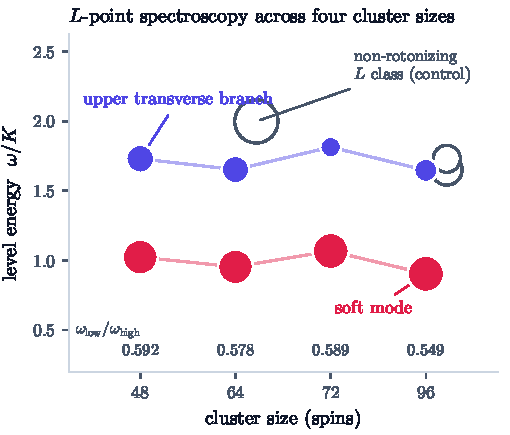
\includegraphics[width=\columnwidth]{fig_ladder.pdf}
\caption{\textbf{Finite-size stability and internal controls.}
Filled symbols: lower and upper branches of the reconstructing $L$
class. Open symbols: dominant levels of the inequivalent
nonreconstructing class on the anisotropic 64- and 96-site clusters.
Numbers give $\omega_{\rm low}/\omega_{\rm high}$. The lower branch
retains approximately half of the sublattice-summed weight at every
size.}
\label{fig:ladder}
\end{figure}

\emph{Why there: the Feynman ratio.}---The location of the
reconstruction is not accidental, and it can be anticipated without
computing a single excited state. Two moments of Eq.~(\ref{eq:szz})
are ground-state quantities. The zeroth is the equal-time structure
factor $S(\bq)$, which measures how much static correlation at
wavevector $\bq$ the ground state already contains. The first,
obtained from the double commutator of $S^z(\bq)$ with $H$, is
\begin{equation}
f_1(\bq)=\frac{K}{2N}\sum_p\bigl\langle W_p+W_p^\dagger\bigr\rangle
\sum_\mu\bigl|g^\mu_p(\bq)\bigr|^2,
\label{eq:f1}
\end{equation}
where $g^\mu_p(\bq)$ is the alternating lattice curl of the
sublattice-resolved electric-field wave around plaquette $p$.
Equation~(\ref{eq:f1}) has the form of a Maxwell magnetic energy: a
purely geometric factor, the squared curl of the imposed wave,
weighted by the measured ground-state ring coherence. It is the
oscillator strength---the energy cost of creating the electric-field
wave---and it contains no fitted parameter.

Their ratio $f_1/S$ is the variational energy of the single-mode state
$S^z(\bq)|0\rangle$, and equivalently the centroid of the spectrum
that state creates. This is Feynman's construction for the helium
roton~\cite{Feynman1954}: a collective excitation is cheap where the
probe couples weakly and the static correlations are already strong.
Two features make it useful here. It is an upper bound on the lowest
excitation in the channel, so a small value certifies softness; and
because both factors come from the ground state, it can be evaluated
\emph{in advance} and tested as a forward prediction. A low centroid
does not by itself prove a sharp pole---that is what the
diagonalizations supply---but it says where to look.

It succeeds three times. On 64 sites the two inequivalent $L$ classes
have $S=0.369$ and $0.227$; the lower-ratio class develops the
$0.954K$ level with $50.0\%$ of the weight, while the other stays
dominated by a $1.998K$ level with $77\%$. On 96 sites, with
$S=0.355$ and $0.241$, the test repeats. On 72 sites the ratio at $L$
and at $(\frac16,\frac12,\frac12)$ differ by $0.9\%$, and the two
soft levels then appear within $0.7\%$, at $1.068K$ and $1.075K$ with
$54\%$ and $55\%$ of their respective weights. The ratio does not
predict absolute pole energies---the centroid also carries the
high-energy weight---but it identifies which momenta reconstruct.

Both factors conspire at $L$. Geometrically, for $\bq\parallel[111]$
one family of hexagons lies in the wavefronts of the electric-field
oscillation and its alternating curl vanishes identically: the
family-resolved geometric weights are $(96,96,96,0)$ at $L$ against
$(96,96,96,96)$ at $X$, reducing $f_1$. Geometry alone is
insufficient, since the same cancellation occurs at shorter
wavelength along $[111]$ where nothing anomalous happens. The second
ingredient is dynamical: at 48 sites $S(L)=0.370$, whereas the
equal-amplitude superposition over the same configurations gives
$0.297$ and classical loop Monte Carlo on a 2048-site ice manifold is
flat among zone-boundary momenta. The enhancement is made by the
interacting quantum amplitudes, not by the ice constraint---which is
what distinguishes this from a Rokhsar--Kivelson resonon, whose
softening follows directly from classical correlations.

Because $f_1/S$ needs only the ground state, it can be evaluated far
beyond exact diagonalization. The ring Hamiltonian is stoquastic in
the ice basis, permitting sign-free Green's-function Monte Carlo with
forward walking, benchmarked against the exact 48-site $S(L)$ to
every digit. On complete allowed momentum grids of $864$ and $2048$
spins the ratio at $L$ is $2.142(10)$ and $2.179(19)$, against
$2.660(10)$ and $2.713(21)$ at $X$ and $2.72$--$2.78$ at $W$, $K$,
and $U$: an $L$-centered minimum $20$--$25\%$ deep that drifts by
$1.7\%$ between the two sizes (Fig.~\ref{fig:thermo}). The softness
extends along a shallow $(t,\frac12,\frac12)$ valley, which is why
the 72-site cluster finds a second reconstructed momentum on that
line.

\begin{figure*}[t]
\centering
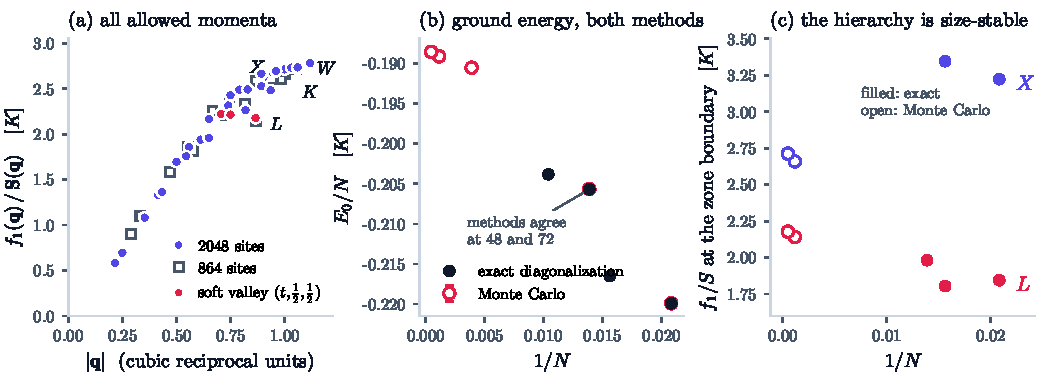
\includegraphics[width=0.98\textwidth]{fig_thermo.pdf}
\caption{\textbf{Large-system ground-state landscape.}
(a) $f_1(\bq)/S(\bq)$ on the 2048-site supercell grouped by geometric
role, with each group's $|\bq|$ range indicated; interior stars lie
below the boundary plateau only because the centroid is still rising
with $|\bq|$, and at matched $|\bq|=0.75$ the valley sits $9$--$10\%$
below the interior star $(0,0,\frac34)$. Open squares: 864-site
values at shared momenta. (b) Ground-state energy from exact
diagonalization and Monte Carlo, agreeing where both exist.
(c) Size evolution at $L$ and $X$ across both methods.}
\label{fig:thermo}
\end{figure*}

\emph{Interpretation.}---The phenomenology is that of a roton in
Feynman's sense: a weight-dominant collective excitation at finite
momentum, located by the ratio of oscillator strength to static
correlation, and lowered further by correlated relaxation. That the
designation belongs to the lower branch is measured rather than
assumed. The single-mode state built from $S^z(\bq_L)|0\rangle$
overlaps the lower-branch multiplet with squared amplitude $0.88$,
$0.87$, and $0.86$ on the 48-, 64-, and 72-site clusters, coupling to
the upper branch only through the orthogonal transverse channel: the
Feynman construction produces this branch, not the other. Relaxing
that state within the exact spectrum recovers $28$--$32\%$ of its
energy, a size-stable amount, through a strongly family-selective
reorganization of ring coherence.

We state the limits precisely. The lattice modifies the geometry of
the phenomenon: along the radial $[111]$ direction the centroid rises
from $\Gamma$ to $L$ and folds back by periodicity, so there is no
helium-like radial dip; the minimum lives in the zone-boundary
manifold, where the competing short-wavelength excitations are. The
finite-size branch descends into the zone boundary while the
large-system centroid develops its minimum there. Sharpness is
established up to 96 spins; beyond that the Monte Carlo constrains
the centroid, not the pole, and whether the level broadens into a
narrow continuum in the thermodynamic limit is open. Finally, the low
mode is not a multiparticle state of the free theory: it is odd under
spin reversal, excluding even photon numbers, and at $1.02K$ it lies
a factor of five below the three-photon threshold of $5.55K$
computed on the same torus---an exclusion valid for weakly
renormalized constituents, which we do not extend further.

\emph{Experimental implications.}---The signature is a two-feature
zone-boundary response where a renormalized photon would give one.
Following the $[111]$ direction outward, a single dispersing mode at
small $\bq$ should separate into two, the splitting growing from
unresolvable to nearly a factor of two by the zone boundary, with the
\emph{lower} feature carrying two to three times the weight of the
upper. Two aspects of this are scale-free and therefore testable
without knowing $K$: the ratio of the two energies, $0.55$--$0.59$,
and the ratio of their weights. A single photon branch with a
renormalized velocity, however strongly renormalized, produces
neither. Because the reconstruction tracks $f_1/S$ rather than the
label $L$, the same signature should appear along the
$(t,\frac12,\frac12)$ line, as it does in our 72-site spectrum.

Two caveats bound this. A material-specific neutron cross section
reweights the sublattice amplitudes coherently, so the theoretical
$50$--$54\%$ fraction should not be read as a universal neutron
intensity; and longer ring exchanges, virtual spinons, and other
microscopic terms can modify the zone-boundary spectrum of a real
material. The robust prediction of the minimal model is the
redistribution itself.

\emph{Discussion.}---The emergent photon of quantum spin ice is
nonperturbatively reconstructed at the lattice scale. Half of the
longitudinal spectral weight moves into a mode near $1K$ whose
scale-free ratio to its photon-like partner is stable across four
clusters; the mode is microscopically distinguished by its
flippability response, and its location follows a ground-state
diagnostic that we verify predictively and carry to $2048$ spins.
What makes this possible is that the compact theory has no small
parameter at short wavelength: the saturated electric field forbids
increasing the amplitude of a field wave, so a finite-amplitude
excitation must rearrange which bonds carry the two allowed values,
and that rearrangement is cheapest where static correlations are
strongest and the curl is weakest.

The broader implication is that the short-wavelength dynamics of a
compact spin-$\frac12$ gauge field are qualitatively richer than a
weakly renormalized Maxwell photon. The obvious next questions are
whether the reconstruction survives virtual spinons and longer ring
exchanges in microscopic XXZ models, and whether the finite-size pole
remains sharp in the thermodynamic limit---a question that requires
dynamical rather than ground-state Monte Carlo.

\begin{acknowledgments}
We thank the Digital Research Alliance of Canada for computational
resources. The complete set of scripts generating the numerical
results and figures is included with the submission.
\end{acknowledgments}

\bibliographystyle{apsrev4-2}
\bibliography{refs}

\end{document}
